\documentclass[a4paper]{article}
\usepackage[left=3cm, right=3cm]{geometry}
\usepackage{hyperref}
\usepackage{cite}
\usepackage{amssymb}
\usepackage{url}
\usepackage{float}
\usepackage{longtable}
\usepackage{array}
\usepackage{algorithmic}
\usepackage[boxed]{algorithm}
\usepackage{color}
\usepackage{graphicx}
\usepackage{tabularx}
\usepackage{caption,subcaption}
\pagestyle{headings}
\newcommand{\secondo}{\textsc{Secondo}}
\newcommand{\bmodb} {BerlinMOD Benchmark}
\newcommand{\op}[1]{\textbf{#1}}
\newcommand{\dt}[1]{\textsl{\underline{#1}}}
\newcommand{\true}{\textsl{TRUE}}
\newcommand{\false}{\textsl{FALSE}}
\newcommand{\secver}{2.9.StableNewFlob}
%opening
\title{Network Data Model and BerlinMOD Benchmark}
\author{Simone Jandt}
\date{Last Update: \today}
\begin{document}
\maketitle
\begin{abstract}
In the past several data models for the representation of histories of  spatio-temporal data
objects have been developed. Among others we can categorize these data models
into data models for objects moving freely in the two dimensional space and data
models for network constrained moving objects. In this paper we select two representatives,
one for each data model category, which are both implemented in the \secondo{} DBMS,
and compare their capabilities with the \bmodb{}. We describe the translation
from the \bmodb{} into the network constrained data model and show
that in our experiments the network constrained data model outperforms the data
model of free movement in the two dimensional space by orders of magnitudes.
%The very good results of the network data model in this comparison encourages us
%to propose a extension of the \bmodb{} with a additional query set BerlinMOD/Net.
%This new query set covers the specialised challenges for network constrained
%data models and enables us to use the \bmodb{} to compare the capabilities of
%different network data models with respect to this specialised network challenges.
\end{abstract}
\section{Introduction}
In the past several data models for the representation of spatial and
spatio-temporal data objects have been developed. Among others we can categorize
them into data models for objects moving freely in two dimensional space and
data models for network constrained moving objects. For both categories
several different data models have been presented like
\cite{chenzaniolosqlst,335426} for spatio-temporal data objects moving freely in
two dimensional space and \cite{1146465,956692,VazWolfNetMod} for
spatio-temporal data objects that are constrained by given networks,
to name just a few. Objects which are restricted to use existing networks, like
cars are restricted to use road networks, can be represented as moving point object
in both data
models, while objects, which are not restricted by a given network, like people,
can be represented as moving point object only in a data models of free movement
in space.

But if everything can be represented by a data model of free movement
space why do we spend time on network data models? Now, our experiments
presented in this paper show that the network data model outperforms the data model of
free movement in two dimensional space significantly. The network data model uses
less than 60\% of the storage space of the data model of free movement in space, mostly caused
by the fact that the number of units for the moving point objects in the network
data model is less than 50\% of the number of units in the data model of free
movement in two dimensional space. The total run time of the \bmodb{} for the
network data model is less than 50\% of the total run time of the data model of
free movement in two dimensional space. We think that this results show that
it is useful to develop specialised data models for specialised data structures
like network data models for network constrained moving objects to save storage
space and reduce query run times.

For this paper we choosed two representatives one for each data model category.
Both representatives are available in the \secondo{} DBMS and use the same
temporal representation. So we can exclude that different DBMS or temporal
representation issues bias the results of our data model comparison.

The network constrained data model is represented by
the network data model presented in \cite{1146465} and the data model of free
movement in two dimensional space is represented by the data model presented in
\cite{335426}.

For us it seems logical to use the \bmodb{} \cite{BerlinMODVLDB} which is also
available in the \secondo{} DBMS to compare the capabilities of the
both data models. The \bmodb{} is best to our knowledge the first benchmark for
complete spatio-temporal database systems and it is developed in the \secondo{}
DBMS. Furthermore the data generated by the \bmodb{} data generator is restricted
to the streets of the German capital Berlin, such that it can be translated into
a network constrained environment. And not at last the data model used in the
\bmodb{} is the data model of free movement in two dimensional space that we use
for our comparison. So we only have to translate the spatial and spatio-temporal
data types of the \bmodb{} once into our network data model representation.
This simplifies the control of the query results and avoids errors caused by
translation errors.

The translation of the spatial and spatio-temporal data types of the \bmodb{} data
into the network data model representation described in this paper can be seen as
example for the usage of the \bmodb{} with other compatible data representations or
DBMS.

%The very good results of the network data model encourages us to propose the extension
%of the \bmodb{} by a query set BerlinMOD/Net. The new query set covers the specialised
%challenges of network data models like network distance computing which are not
%covered by the original \bmodb{}. The new query set should enable us to compare
%the capabilities of different network data models with respect to the special
%challenges of network constrained data models.

The rest of the paper is organised as follows: In section \ref{sec:relWork} we give a
short reminder of the underlying \secondo{} DBMS (\ref{sec:secondo}), the \bmodb{}
(\ref{sec:bmodb}) and the two data models (\ref{sec:bmodbdatamod}
and \ref{sec:netdatamod}) we choose as representatives for our comparison.
The translation of the \bmodb{} data and query set in the network data model
representation is described in section \ref{sec:Translation}. The resulting
experimental benchmark setup is described in section \ref{sec:scenario} followed
by the results of our experiments in section \ref{sec:results}.
%At least we present our proposed extension of the \bmodb{} for network data models in
%section \ref{sec:newqueries}.
We conclude our work in section \ref{sec:summary}.
\section{Related Work}
\label{sec:relWork}
In the past other data models for free movement in the space
\cite{chenzaniolosqlst,335426} and for network constrained movement have been
presented \cite{1146465,956692,VazWolfNetMod}. As well there are some more
benchmarks \cite{COSTBenchmark, QueriesTheodoridis} and database systems for
spatial and spatio-temporal data types \cite{1054151,HERMES}. But best to our
knowledge they don't actually provide a combination of different implemented
and supported data models together with a existing benchmark feasible for moving
objects in space and network constrained moving objects like the actual
\secondo{} DBMS. So it is self-evident for us to use the \secondo{} DBMS in
combination with the provided data models and the \bmodb{} to compare the
capabilities of the network constrained data model and the data model of free
movement in two dimensional space provided with the \secondo{} DBMS.

In the next subsections we give short reminders of the \secondo{} database system
(\ref{sec:secondo}), the \bmodb{} (\ref{sec:bmodb}), and the both data models
(\ref{sec:bmodbdatamod}, \ref{sec:netdatamod}) we used in our experiments.
\subsection{Secondo}
\label{sec:secondo}
The extensible \secondo{} DBMS presented in \cite{686903,1054151} provides a
platform for implementing various kinds of data models. It provides a clean
interface between the data model independent system frame and the content of the
single data models. Hence \secondo{} can be easily extended by the user
implementing algebra modules to introduce  new data types and operations on
this data types. The user may define additional viewers for the graphical user
interface or write additional optimization rules or cost functions to extend the
the optimizer. Since \secondo{} version 2.9 the user may publish his extensions
as \secondo{} plugin such that other users can use this plugin to extend their own
\secondo{} system to use the new provided functionalities or repeat the published experiments.
\secondo{} is free available in the web \cite{secondoweb} and comes with a number
of already implemented spatial and spatio-temporal data types
and operations including the spatio-temporal data model of free movement in the
two dimensional space \ref{sec:bmodbdatamod} and the network data model
\ref{sec:netdatamod} used in this paper. Furthermore the \bmodb{} described in
\ref{sec:bmodb} has been developed in the \secondo{} DBMS. For our experiments
we used the \secondo{} version \secver{}.
\subsection{BerlinMOD Benchmark}
\label{sec:bmodb}
The \bmodb{} was presented in \cite{BerlinMODVLDB} \nocite{BerlinMOD} and the
provided scripts for the data generator are implemented as \secondo{} DBMS operations.
The \bmodb{} is available in the web \cite{berlinmodweb} and provides a well defined
data-set and queries for the experimental evaluation of the capabilities of
spatial and spatio-temporal database systems dealing with histories of moving
objects. The \bmodb{} emphasises the development of complete systems
and simplifies experimental repeatability pointing out the weakness and the potency's
of the benchmarked systems.

The data-sets of the \bmodb{} are created using the street map of the German
capital Berlin \cite{bbike} and statistical data about the regions of Berlin
\cite{bevberlin,berlinstadtatlas} as input relations.
The created moving objects represent cars driving in the streets of Berlin,
simulating the behaviour of people living and working in Berlin.
Every moving object has a home node and a work node. Every weekday each car will
do a trip from the home node to work the work node in the morning and vice versa
in the late afternoon. Beside this randomly chosen cars will make additional
trips in the evening and up to six times at the weekend to randomly chosen
targets in Berlin and back home. The \bmodb{} uses the data model of free movement in two
dimensional space described in section \ref{sec:bmodbdatamod}. Because the \bmodb{}
generates all data sets restricted to the street map of Berlin the \bmodb{} can
also be used for network constrained data models, if the spatial and spatio-temporal
data types are translated into a corresponding network data model, like we did
for our experiments.

The number of observed cars and the duration of the observation period can be
influenced by the user setting the $scalefactor$ to different values in the data
generation script of the \bmodb{}. For example at $scalefactor$ 1.0 the data generator
creates 2000 moving point objects observed for 28 days. Each of them sending a
GPS-signal every 2 seconds. This simulated signals are simplified such that time
intervals when a car doesn't move or moves in the same direction at the same
speed are merged into one single time interval. For example: If a car parks in front
of the work node for 8 hours there will be only one entry in the history of the
cars movement with a time interval of 8 hours instead of 14.400 entries
one for each GPS time interval.

The \bmodb{} provides two different approaches to store the histories of moving
objects. On the one hand the object-based approach (OBA) and on the other hand
the trip based approach (TBA).

In the OBA the complete history for each moving object is kept together into
one single entry. There is only one relation $dataScar$
containing one tuple for each object consisting of the spatio-temporal data of
the object $journey$, the $licence$, the $type$, and the $model$ of the object.

In the TBA we have two relations $dataMcar$ and $dataMtrip$. $dataMcar$ contains
the static data for each object like $licence$, $type$, and $model$ together with
an object identifier $moid$. $dataMtrip$ contains for each $moid$ several tuple
each of them containing all units of a single trip of the moving object or a
single unit for a longer stop. For example each time the car drives from home node
to work node is a single trip and each time the car parks in front of the office
is also a single trip.

Beside the moving point objects the \bmodb{} provides several data sets each of them
containing 100 pseudo randomly generated data objects which are used in the
benchmark queries. Table \ref{tab:queryobjects} gives an overview of this query
objects. The \bmodb{} deals also with subsets from this query object sets consisting
of the first or second 10 query objects of a query object set. They are labeled
by the name of the query object set followed by a 1 for the first 10 or a 2 for
the second 10 query objects of the query object set.

\begin{table}[H]
  \begin{tabularx}{1.0\textwidth}{|l|X|}
    \hline
    \textbf{Name of Data Set}&\textbf{Tuple Content}\\
    \hline
    $QueryPoints$&Object identifier and \dt{point} values.\\
    \hline
    $QueryRegions$&Object identifier and \dt{region} value.\\
    \hline
    $QueryInstants$&Object identifier and time stamps.\\
    \hline
    $QueryPeriods$&Object identifier and space of time.\\
    \hline
    $QueryLicences$& Object identifier and a \dt{string} representing a licence value.\\
    \hline
  \end{tabularx}
  \caption{Query Object Relations of \bmodb{}}
  \label{tab:queryobjects}
\end{table}

The \bmodb{} provides two sets of queries BerlinMOD/R and BerlinMOD/NN.
BerlinMOD/R addresses range queries and BerlinMOD/NN nearest neighbour queries.
In this paper we will focus on the range queries, which are the main aspect of the
\bmodb{} up to now.

The query set BerlinMOD/R includes 17 queries selected of the set of possible
combinations of the 5 aspects:
\begin{itemize}
  \item known or unknown object identity,
  \item standard, spatial, temporal, or spatio-temporal dimension,
  \item point, range, or unbounded query interval,
  \item single object or object relations condition type,
  \item with or without aggregation.
\end{itemize}
We will present the 17 queries in more detail in section \ref{sec:queries}
together with our network data model algorithms for this queries.
\subsection{Data Model of Free Movement in two dimensional space}
\label{sec:bmodbdatamod}
The data model used by the \bmodb{} is the same data model of free movement in
two dimensional space presented in \cite{594784,335426,352963}. Spatial
positions are assumed to be located into a two dimensional space. A single spatial
position is represented by the data type \dt{point}. A \dt{point} consists of a pair of
\dt{real} values interpreted as x,y-coordinates in the assumed two dimensional plane.

Streets are represented by \dt{line} values. A \dt{line} value consists of a set
of $half segments$ representing the geometry of the line in the two dimensional space.
Each $half segment$ consists of two \dt{point} values and a Boolean flag telling us
if the left or the right point is the dominating point of the $half segment$.

Regions are represented by the data type \dt{region}. A \dt{region} consists of
a set of $half segments$ defining the outer border of the region in
the two dimensional space. If a region contains wholes the inner border is also
formed by the $half segments$.

In \secondo{} all this spatial data types and many standard data types can be
lifted to become time dependent \dt{moving} values. For all data types \dt{$\alpha$}
the constructor \dt{moving} creates a new data type \dt{moving}(\dt{$\alpha$})
(short form \dt{m$\alpha$}).

A car may be represented by a \dt{moving}(\dt{point}) short \dt{mpoint}.
A \dt{mpoint} consist of a set of units called
\dt{unit}(\dt{point}) (short form \dt{upoint}). Each \dt{upoint} consists of a time
interval and two \dt{point} values. The first \dt{point} value represents the
position of the \dt{mpoint} at the start of the time interval and the second
\dt{point} value represents the position of the \dt{mpoint} at the end of the
time interval. It is assumed that the object represented by the \dt{mpoint}
moves on the straight line between this two points with constant speed within the
given time interval. The velocity of the object is given by the ratio from the
distance of the two points and the length of the time interval of the unit.
All units of a \dt{mpoint} must have disjoint time intervals, because a car
cannot be at two different positions at the same time.
The units are sorted by ascending time intervals.

This spatio-temporal data model of \dt{moving} allows us to compute the position
of a \dt{mpoint} at every time instant within its definition time.
We can also compute the time instant the point passed a
given position assumed the \dt{mpoint} ever passes this position. The position of a
\dt{point} at a given time instant is represented by a \dt{intime}(\dt{point})
(short form \dt{ipoint}). A \dt{ipoint} consists of a time instant and a \dt{point} value.

Some other data types of \secondo{} which are used in the \bmodb{} are shown in
table \ref{tab:bmodbdatatypes}.
\begin{table}[H]
\begin{center}
\begin{scriptsize}
\begin{tabularx}{1.0\textwidth}{|l|X|}
\hline
\textbf{Data Type} & \textbf{Description} \\
\hline
\dt{bool} & Usual boolean data type.\\
\hline
\dt{int} & Usual integer number.\\
\hline
\dt{real} & Usual real number.\\
\hline
\dt{instant} & A point in time.\\
\hline
\dt{periods} & A set of disjoint and not connected spaces of time.\\
\hline
\dt{mbool} & A time dependent boolean value, which will be constant \true{} or \false{}
within each \dt{ubool} \\
\hline
\dt{mreal} & Time dependent real number. Each unit will be defined by a function
of time representing the \dt{real} value at each time instant.\\
\hline
\end{tabularx}
\end{scriptsize}
\caption{Other Data Types of \bmodb{}}
\label{tab:bmodbdatatypes}
\end{center}
\end{table}
\subsection{Network Data Model}
\label{sec:netdatamod}
The central idea of the network data model presented in \cite{1146465} is that
every movement is constrained by a given network and every position can be described
relative to this network. The data type \dt{network} is the central
data type in the network data model. All other data types of the network data model
are related to a given \dt{network} object by the unique network identifier that
is part of each \dt{network} object.

The \dt{network} object contains all spatial information of the represented network.
The \dt{network} consists of three main relations ($routes$, $junctions$, and $sections$),
two arrays providing fast access to adjacent network sections,
and some B-Tree and R-Tree indexes to supporting faster access to the main relations.

The relation $routes$ of the \dt{network} contains the attributes of the
streets like $id$, $route curve$, $route length$, and two Boolean flags. The first
flag indicates if the route starts at the lexicographically smaller end point or not.
The second flag indicates if the lanes of the street are separated like on German
Highways or not.

The $junctions$ relation of the \dt{network} contains all attributes of the street
crossings like the two route identifiers of the first and second street meeting at the
crossing, the distance of the crossing from the start of the first respectively
second street, tuple identifiers of the both streets in the routes relation,
tuple identifiers of the sections connected by this junction in the sections relation,
and a connectivity code telling us which lanes of the two streets are connected
by the crossing.

The $sections$ relation of the \dt{network} object contains the
attributes of the street parts between two crossings or a crossing and
the end of the street. This are the route identifier of the street the section
belongs to, the tuple identifier of this street in the routes relation, the start
position and end position of the section on the street, the section curve, and
again two Boolean flags with the same meaning as in the routes relation.

Furthermore there are two arrays in the \dt{network} object providing a fast
access from each section to their adjacent sections with respect to the driving
direction. Two sections are adjacent if their lanes are connected by a junction.

We created four B-Tree indexes for the route identifier attributes in the $routes$,
$junctions$ and $sections$ relation, and a R-Tree index over the curve attribute
of the $routes$ relation to support faster execution of operations dealing with
the relations of the \dt{network} object.

The data type \dt{gpoint} represents single positions in a given network. Besides the
network identifier a \dt{gpoint} consists of a route identifier, a distance from
the start of the route to the position of the \dt{gpoint} and a $side$ value
({$up$, $down$, $none$) telling us if the position is reachable from the $up$
or the $down$ side of the route in case of separated lanes. For simple
streets or positions which are reachable from both sides of the route the side
value is always $none$.

Parts of the network, regardless if they represent paths or regions, are given as
\dt{gline} values. Besides the network identifier a \dt{gline} consists of a set
of $route interval$s, and two Boolean flags. The Boolean flags tell us if the
\dt{gline} is defined and if the set of $route interval$s is sorted.

Each $route interval$ consists of a route identifier identifying the route
the route interval belongs to, and the start and the end position from the
route interval on this route
\footnote{In the original paper the $route interval$ includes a $side$ value
analogous to the \dt{gpoint}. But this parameter is not part of the implementation yet.}.
We call a \label{sec:sortedgline} set of $route interval$s sorted if the following
conditions are fullfilled:
\begin{itemize}
	\item all $route interval$s are disjoint
	\item the $route interval$s are stored in ascending order of their route identifiers
	\item if two disjoint $route interval$s have the same route identifier the
$route interval$ with the smaller start position is stored first
	\item for all $route interval$s the $start position \le end position$
\end{itemize}
Many algorithms take profit from sorted \dt{gline} values. For example: If $n$
is the number of the route intervals in a \dt{gline} the
decision, if a \dt{gpoint} is inside the \dt{gline} needs O($n$) time for unsorted
and O($\log n$) time for sorted \dt{gline} values,

Unfortunately not all \dt{gline} values can be stored sorted. If a \dt{gline}
value represents a path between two \dt{gpoint} in the network, we need the
route intervals exactly in the sequence they are used in the path. This will
nearly never be a sorted set like defined before.  We store \dt{gline}
values sorted whenever this is possible to support faster query execution, and
introduced a Boolean sorted flag. Every algorithm which deals with \dt{gline} values
checks this flag and uses the corresponding code.

Mostly similar to the \dt{mpoint} of the other data model there is a
\dt{mgpoint} in the network data model. A \dt{mgpoint} consists of a set of
\dt{ugpoint} with disjoint time intervals. Each \dt{ugpoint} consists of a time
interval and two \dt{gpoint} values. Every time the \dt{mgpoint} changes the route
or the speed a new \dt{ugpoint} is written. Each \dt{ugpoint} is assumed to follow
the same route from the start to the end position at the same speed. So accordingly
to the \dt{mpoint} we can compute the network position of the \dt{mgpoint} at every
time instant within the definition time of the \dt{mgpoint} as \dt{intime}(\dt{gpoint}).

In deviation from the original network data model we extended the implementation
of the \dt{mgpoint} with four additional attributes to support faster query execution:
\begin{enumerate}
	\item The total driven distance
	\item A sorted set of $route interval$s representing the positions ever
traversed by the \dt{mgpoint}
	\item A Boolean defined flag for the set of $route intervals$
	\item A spatio-temporal minimum bounding box
\end{enumerate}
The sorted set of $route interval$s was introduced, because analogous to sorted
\dt{gline} values it makes it much faster to decide if a \dt{mgpoint} ever passed
a given network position or not. Instead of a linear check of all $m$ \dt{ugpoint}s
of a \dt{mgpoint} we can perform a binary scan on the much lower number $r$ of the passed $route interval$s.
This reduces the time complexity from O($m$) to O($\log r$) for the \op{passes}
operation. Logically the set of $route interval$s should be a sorted \dt{gline}
value but the \secondo{} DBMS restricts us to use a sorted set of $route interval$s
instead.

The spatio-temporal minimum bounding box was introduced as parameter to the
\dt{mgpoint} because the computation of this value is very expensive in the
network data model. Although each unit of a \dt{mgpoint} stays on the same route
at same speed it may follow different spatial directions. For example a route may
lead uphill in serpentine. A spatial bounding box only computed from the spatial
start and end position may not enclose all spatial positions of the car within
the unit. Therefore we have always to examine the spatial dimensions of the
$route interval$ passed within a unit to compute the units bounding box. This
needs a access to the route curve in the $routes$ relation of the corresponding
\dt{network} object. If $r$ is the number of routes
of the network and $h$ the number of $half segments$ belonging to the $route interval$
passed in a unit we need O($h + \log r$) time to
compute the bounding box for a single unit. The bounding box of the \dt{mgpoint}
is the union of the bounding boxes of its $m$ units. So the computation of the
spatio-temporal respectively spatial bounding box of a \dt{mgpoint} needs
O($m(h + \log r)$) time. This very expensive computation is only done
on demand or if we can get the bounding box for free. For example we can copy
the bounding box of a \dt{mpoint} at the translation time into a \dt{mgpoint}
without big computational costs. The bounding box attribute is not maintained. If
the \dt{mgpoint} value changes the bounding box attribute is set to be undefined
until recomputing is necessary.
\section{Translation of BerlinMOD into Network Data Model}
\label{sec:Translation}
In this section we describe the creation of the \dt{network} object from the $streets$
value of the \bmodb{} in section \ref{sec:createNetwork}. Followed by the
description how to use this new created \dt{network} value as reference for the
translation of all spatial and spatio-temporal data type objects of the \bmodb{}
into the network data model representation in section \ref{sec:translateSTdata}.
In section \ref{sec:createIndex} we describe the indexes we build on the network
data model representation to support faster query execution. We close this part
with section \ref{sec:queries} were we describe the executable \secondo{} queries
for the network data model representation of the \bmodb{}.

Executable \secondo{} scripts for the network and index creation, object translation,
and the network benchmark queries can be downloaded from our website
\cite{berlinmodweb}.
\subsection{Create Network Object}
\label{sec:createNetwork}
The \dt{network} object $net$ is created by extracting the $routes$ data from
the $streets$ object that is created by the BerlinMOD Data Generator.
The extracted data $r$ is used to compute the crossings of the
routes of Berlin $j$. The data source lacks on information about the connectivity
of the street crossings, such that we use the maximum value for the connectivity
code of each crossing as default value in this step.
Now we can use $r$ and $j$ as input relations for the operator \op{thenetwork}
to create our \dt{network} object $net$ representing the streets of Berlin in
the network data model representation of the \bmodb{}.

The network creation algorithm first copies all tuple of $r$ to the
$routes$ relation of $net$ and creates the B-Tree index of the route
identifiers and the R-Tree index of the route curves of the $routes$ relation of
$net$. Then all tuple of $j$ are copied to the $junctions$ relation
of $net$ and the tuple identifiers for the both routes connected
by this junction are added to the junctions entry. After that we build two B-Trees
indexing the route identifiers of the first respectively second route in the
$junctions$ relation. Next for every route of the $routes$ relation all junctions
on this route are taken from the $junctions$ relation to compute the up and
down sections for each of this junctions on the route. The up and down
sections are inserted into the $sections$ relation of $net$ and the
tuple identifiers of the sections are added to the entry of the corresponding
junction in the $junctions$ relation. After that the B-Tree index for the
route identifiers in the $sections$ relation is created and the adjacency
lists of $net$ are filled with the adjacent section pairs defined by the
$junctions$ relation.

If $|r|$ is the number of routes and $|j|$ is the number of junctions.
The algorithm needs O($|r| \log |r|$) time to copy $r$ to the
$routes$ relation of $net$ and create the indexes of the
$routes$ relation. The creation of the $junctions$ relation and the build
of the B-Trees indexes takes O($|j| \log |j|$) time.
O($|r||j|$) time is needed to fill the $sections$ relation and
O($|j|$) time to fill the $adjacency lists$ of $net$. Altogether
the complete algorithm needs:
O($|r| \log |r|+|j| \log |j| + |r||j|$)
time to create the $net$ from the two input relations $r$ and $j$.
\subsection{Translate Spatial and Spatio-Temporal Data Types}
\label{sec:translateSTdata}
In this section we describe the translation of the spatial and spatio-temporal
data types of the \bmodb{} data set into network respectively network-temporal
objects. All translations are done relative to the \dt{network} object $net$ that
we described in section \ref{sec:createNetwork}.
All algorithms in this section get a spatial respectively spatio-temporal \bmodb{}
data type object and the \dt{network} object $net$ as input they return the
corresponding network data model object respectively an undefined network data model
object if the input data object is not constrained by $net$.
\subsubsection{Translate \dt{point} into \dt{gpoint}}
The \op{point2gpoint} operation translates a \dt{point} value $p$ into a corresponding
\dt{gpoint} value $gp$ if possible. This operation is also included in the other translation
operations. The algorithm uses the R-Tree index of the
$routes$ relation of $net$ to select the route curve closest to $p$ and computes the
position of $p$ on this route curve. In case of the \bmodb{} the $side$ value of
$gp$ is always set to $none$, because the \bmodb{} does not differentiate between
the different sides of a street.

If $r$ is the number of routes in the $routes$ relation
and $k$ is the number of possible candidate routes the worst case complexity
of the algorithm is O($\log{r} + k$).

This should be all to translate the \dt{point} values of the $QueryPoints$
relation of the \bmodb{} into network query positions. But there is a problem with
the network data model representation of junctions. In the network data model
contrary to the data model of free movement in the two dimensional space each junction
has more than one \dt{gpoint} representation, because each junction is related to
two or more routes. Hence if a junction position is given related to route $a$
we won't detect the junction as passed if a \dt{mgpoint} object passes the junction
on route $b$ in all cases, because the definition of \op{passes} in the network
data model is slightly different from the \op{passes} operation in the \bmodb{} data model.
Unfortunately all query points of the \bmodb{} are junctions. To make the results
comparable we added a operator \op{polygpoints}, which returns for every input
\dt{gpoint} value $gp$ a stream of \dt{gpoint} values. If $gp$ represents a junction
we return all \dt{gpoint} values representing the same junction in $net$,
otherwise we return only $gp$ in the stream. So we got 221 query \dt{gpoint}
values in $QueryPointsNet$ for the 100 query \dt{point} values in
$QueryPoints$ and 22 \dt{gpoint} values in $QueryPoints1Net$ for the
10 \dt{point} values of $QueryPoints1$ of the \bmodb{}. This means we have
always to compute the results for the doubled number of query points in our network
data model than in the data model of free movement in space.
\subsubsection{Translate \dt{mpoint} into \dt{mgpoint}}
The second operation \op{mpoint2mgpoint} translates a \dt{mpoint} value $s$
into a \dt{mgpoint} value $t$. The main idea of the algorithm is to use the
continuous movement of $s$ to reduce computation time. We initialize the
algorithm by reading the first unit of $s$ and use the \op{point2gpoint}
algorithm to find a route in the network containing the $start$ and
the $end point$ of this unit. We initialize the first unit of $t$ with
the computed network values. Then we read the next unit of $s$ and try to find
the $end point$ of the new unit on the same route the last unit of $s$ was
found. If the $end point$ is found on the same route we check the moving direction
on the route and speed of the point in the unit. If they are equal to the actual unit we extend
the actual unit of $t$ to enclose the value of the actual unit of $s$. If the
speed or the moving direction on the route changes we write the actual unit to $t$ and initialize
a new unit for $t$ with the network values of the actual unit from $s$.
If the $end point$ can't be found on the same route than the last unit from
$s$ we write the actual unit of $t$ and start a search on the route curves
of the adjacent sections to find the route curve that contains the $start$
and the $end point$ of the actual unit of $s$. We initialize a new unit
for $t$ with the estimated network values for the actual unit of $s$ and
continue with the next unit of $s$. At last we add the actual network unit
to $t$.

The time complexity to find the start values for the first unit is O(\op{point2gpoint}).
For the next $m$ units of $s$ the time complexity is O(1) if $s$ don't change the
route. And O($a$) if the end point is on another route and $a$ is the maximum
number of adjacent sections. So we get a worst case time complexity of
O(O(\op{point2gpoint}) + $ma$) for the translation of a \dt{mpoint} $s$ into a
\dt{mgpoint} $t$.
\subsubsection{Translate \dt{region} into \dt{gline}}
The translation of the \dt{region} values in the $QueryRegions$ relation of the
\bmodb{} into \dt{gline} values of our network data model is done in several steps.
First of all we build a single big \dt{line} object containing all network streets.
Then we compute for each \dt{region} of the $QueryRegions$ the intersection with
this big \dt{line} object. At last we translate the resulting \dt{line} objects
of the intersection, each representing one \dt{region} of the $QueryRegions$
relation, into sorted \dt{gline} values using the \op{line2gline} operation.

The algorithm of the \op{line2gline} operation takes each $half segment$ of a
\dt{line} value and computes a corresponding network $route interval$ by
searching a common $route curve$ for the $start$ and the $end point$ of the
$half segment$ using the \op{point2gpoint} operation. The computed
$route interval$s are sorted, merged and compressed before the resulting
\dt{gline} value is returned. If the number of $half segment$s of a \dt{line}
value is $h$ and the number of resulting compressed $route interval$s is $r$
we get a time complexity of O($h$O(\op{point2gpoint})$+ h \log r + r$) for the
whole algorithm. Whereby the summand $h \log r + r$ is caused by the compressing
and sorting of the resulting \dt{gline} but as mentioned before
in \ref{sec:sortedgline} we think this time is well invested, because it is needed
once and the sorted \dt{gline} value is used many times.
\subsection{Create Indexes on Network Data Model}
\label{sec:createIndex}
For the use with the \bmodb{} we created the following indexes on the network
data model representation of the \bmodb{} data sets:
\begin{itemize}
  \item B-Tree indexes for the $licences$ and $moid$ attributes of the relations
$dataSNcar$, $dataMcar$, and $dataMNtrip$. This indexes are similar to the indexes
created in the \bmodb{} for $dataSCcar$, $dataMCcar$, and $dataMCtrip$, because
the relations $dataSNcar$, $dataMcar$ and $dataMNtrip$ contain the network
data model representation of the $dataScar$, $dataMcar$ and $dataMtrip$ relation
of the \bmodb{}. We don't explain them in more detail.
  \item An R-Tree index of the spatio-temporal bounding boxes of the \dt{mgpoint}
attributes in the $dataMNtrip$ and the $dataSNcar$ relation. Different from the
data model that uses the spatio-temporal units for the spatio-temporal indexes we
used only the big bounding boxes of the whole trips instead of much more small bounding
boxes for each single unit like it is done in the data model of free movement in
two dimensional space.
 \item For every unit of each \dt{mgpoint} we build a three dimensional $netbox$
and for every $route interval$ of every \dt{mgpoint}s trajectory a two dimensional
$netbox$. This $netboxes$ are used to create R-Trees indexing the network and
network-temporal positions of the \dt{mgpoint}s. A temporal-network bounding box
is a degenerated three dimensional rectangle. The coordinates are defined to be
$x_1 = x_2 = route identifier$ as \dt{real} value (The equality of $x_1$ and
$x_2$ makes the degeneration.), $y_1 = \min (star position, end position)$,
$y_2 = \max (start position, end position)$,
and, $z_1 = start time$ as \dt{real} value and $z_2 = end time$ as \dt{real} value.
The network bounding boxes are defined to be degenerated two dimensional rectangles
with x,y-coordinates analogous to the temporal-network boxes.
\end{itemize}
\subsection{Translate Benchmark Queries}
\label{sec:queries}
We developed executable \secondo{} queries for each of the 17 BerlinMOD/R queries
for the object based approach (OBA) and the trip based approach (TBA) using our
network indexes to support faster query execution. The \secondo{} optimizer is not
able to optimize SQL-queries on network data model objects yet, so we tested in
our experiments many different query formulations for each query to get optimal
queries delivering the correct result in a minimum of time.

The limited space does not allow us to show all our executable \secondo{} queries
for the network data model in detail, but they can be downloaded as \secondo{} scripts
from our web page. At this place we give only a short overview over the \bmodb{} queries
and their network data model algorithms.

Every time we need a licence in the result or have a query licence number we need
a additional step in the TBA. Because we have to join the $dataMNtrip$ and $dataMcar$
relation using the $moid$ attribute and the corresponding B-Tree indexes.
We will not repeat this step at every single TBA query description.

Query 1 asks for the models of the cars with licence plate numbers from $QueryLicences$,
and query 2 for the number of vehicles that are ``passenger'' cars. Both queries
deal only with standard attributes so we only changed the relation names and the
B-Tree indexes to match the network data model representation.

Query 3 searches for the positions of the ten cars from $QueryLicence1$ at the
ten time instants from $QueryInstants1$. We use the licence B-Tree to select the
ten cars and computes the positions of these ten cars for each of the ten time
instants from $QueryInstants1$ if the time instant is inside the definition time
of the trip.

In Query 4 asks for the licence numbers of the cars that passed the points
from $QueryPointsNet$. We create a $netbox$ for each \dt{gpoint} in $QueryPointNet$
and use our specialised $netbox$ R-Tree of the \dt{mgpoint} $route intervals$s to
select the vehicles passing the given query points.

The queries 5, 6, and 10 deal with Euclidean Distance values, which are not very
useful in network environments. In networks everything is constrained by the
network and regularly the network distances are computed instead of Euclidean
Distances. We decided to retranslate intermediate results
into spatial respectively spatio-temporal objects and use the existing
Euclidean Distance operation to compute the distances between this objects to make
the results comparable.

Query 5 asks for the minimum distance between places where vehicles with
licences from $QueryLicence1$ and $QueryLicence2$ have been. We select the cars
with licence plate numbers from $QueryLicence1$ respectively $QueryLicences2$ using the
B-Tree over the $Licence$ attribute of $dataSNcar$ relation. In the TBA the
resulting trajectories for each car are aggregated into one single trajectory
for each car. In both approaches we create a \dt{line} value for each resulting
(aggregated) trajectory value of the \dt{mgpoint}s and compute the Euclidean Distance
between this \dt{line} values for each pair of licences one from $QueryLicences1$ and one
from $QueryLicences2$.

Query 6 asks for the pairs of licences from ``trucks`` that have been as close as
10m or less to each other. We filter $dataSNcar$ relation, respectively $dataMcar$
relation to select the ''trucks`` and compute the spatio-temporal bounding box
of each trip of a ''truck``. We extend the spatial dimensions of the bounding boxes
by 5m in each spatial direction and retranslate the \dt{mgpoint} values into \dt{mpoint}
values in a first step. In a second step we compute the \op{symmjoin} of the results from
step one with itself using the intersection of the bounding boxes as join criteria.
We filter the result to include all licence pairs of ''trucks`` that had sometimes
a distance lower than 10m. In the TBA we additionally remove the duplicate licence
pairs from the result.

Query 7 asks for the licence plate numbers of the ''passenger`` cars that reached
the points from $QueryPoints$ first of all ''passenger`` cars during the
observation period. The first step to solve query 7 in the network data model is
equal to query 4. In a filter step we remove all ''not passenger`` cars from the
first intermediate result. We compute for each remaining candidate trip the times
the trip reaches first the query positions. We group the resulting time instants
by the identifiers of the query positions and compute the minimum time stamp of
each group, which is in fact the first time the query position was reached by a
car. In a last step the licences of the ''passenger`` cars reaching the query
positions at this first time instant are computed using the specialised
network-temporal index of the network data model.

Query 8 computes the overall travelled distances of the vehicles from $QueryLicence1$
within the periods from $QueryPeriods1$. We select the candidate cars using the
licence B-Tree, restrict the trips to the query periods and return the lengths of the
trips in the OBA. In the TBA we have to sum up the length of the different
trips driven by a single car within each query period.

Query 9 asks for the longest distance travelled by a single vehicle during each
of the periods from $QueryPeriods1$. We restrict all trips to the periods, compute
the driven distances and select the maximum length for each query periods value.
Again we have to do a additional aggregation of the distances driven from the same
car in the same period in the TBA.

Query 10 asks when and where vehicles with licences from $QueryLicence1$ meet which
other vehicles (distance less than 3m). In the OBA we first retranslate every
\dt{mgpoint} value of $dataSNCar$ into a \dt{mpoint} value and extend the spatial
bounding box of each of this trips by 1.5 m in every spatial direction. After that we
select the ten candidate trips given by $QueryLicences1$, retranslate them and
extend their spatial bounding boxes in the same way. We join all trips from the
first two steps where the extended bounding boxes intersect and filter the
candidate pairs that have different licences and their distance is sometimes
less than 3m to each other. We compute the position of the \dt{mgpoint} at the
times the distance between the remaining candidate pairs of \dt{mpoint} was less
than 3 m and return the licence pairs and the network positions of the first car
when it has been closer than 3 m to the other one.

In the TBA we select the trips given by $QueryLicences1$ from
$dataMNtrip$, retranslate them into \dt{mpoint} values, and extend their spatio-temporal
bounding boxes by 3m in each spatial direction. After that we use the spatio-temporal
index of $dataMNtrip$ to select for each trip of the ten cars, the cars
of $dataMNtrip$ which spatio-temporal bounding boxes intersect the extended spatio-temporal
bounding boxes built before. For every pair of candidate trips we
retranslate the second trip and use the Euclidean Distance function for \dt{mpoint}
values to determine the times when the both \dt{mgpoint} had a distance less than 3m.
At last we restrict the trip of the query \dt{mgpoint} to this times and
aggregate the resulting trips into one single trip for each licence pair.

In our experiments we tried out several indexes to support a faster query execution
of query 10 including the MON-Tree presented in \cite{MONTree}. The MON-Tree showed
very good CPU times but never the less the total run time was very high. In the end
the simple form described above showed the best complete run time performance of all
indexes.

Query 11 asks for the vehicles that passed a point from $QueryPoints1Net$ at one of the
time instants from $QueryInstants1$. We build a network-temporal query box from the
$QueryInstant1$ and $QueryPoints1Net$ relation and use the network-temporal index
on $dataSNcar$, respectively $dataMNtrip$, to select the resulting trips.

Query 12 asks for the vehicles that met at a point from $QueryPoints1Net$ at an time
instant from $QueryInstants1$. The first step of query 12 is identical with query 11.
In a second step the Cartesian Product of the result of the first step with itself
is computed and filtered for vehicles which have been at the same query point
at the same query time instant.

Query 13 asks for the vehicles which travelled within one of the regions from
$QueryRegions1Net$ during the periods from $QueryPeriods1$. We restrict the trips
to the query regions and check if the restricted trips are defined within the query
periods. In TBA possible duplicate licence pairs have to be removed and the
resulting $moid$s must be mapped to the licences of the cars to generate the result
using the B-Tree $moid$ index of $dataMcar$.

Query 14 asks for the vehicles that have been in one of the regions from $QueryRegions1Net$
at a time instant from $QueryInstants1$. We build temporal-netboxes from the query
objects to select candidate trips using the temporal-network position index. We refine the
result filtering the candidate trips really full filling the query predicates.

Query 15 asks for the vehicles passing a point from $QueryPoints1Net$ during a period
from $QueryPeriods1$. Analogous to query 14 we build temporal-netboxes of the
of the query parameters to select the candidate trips using the temporal-network
position index and refine the result filtering the candidates really full filling
the query constraints.

Query 16 asks for the licence pairs one from $QueryLicence1$ and one from $QueryLicence2$
of vehicles, which were both present in a region from $QueryRegions1Net$ within a period
from $QueryPeriods1$, but did not meet there and then. We select the candidate trips
using the licence B-Tree of $dataSNcar$ relation and restrict the resulting trips to be
\op{present} during the query periods and \op{inside} the query region. This is done
one time for the licences from $QueryLicences1$ and one time for the licences from
$QueryLicences2$. The both intermediate results are joined and filtered to get the
trips of different cars which where at the same period in the same region
without meeting each other there and then. In the TBA we have
to do a additional selection from trips with the $moids$ belonging to the cars
selected before by the licences and remove duplicates of licence pairs from the
same period and region.

Query 17 asks for the points from $QueryPointsNet$ that have been visited by a
maximum number of different vehicles. In a first step we use almost the query
algorithm from query 4 to select the trips passing a given query
point. After that we group the cars passing query points by the ids of the
query points and count the number of cars passing this query point. In a last
step the point(s) with the maximum number of passing cars is(are) selected.
In the TBA we have to remove duplicate vehicles from the result list before we
count the number of passing cars.
\section{Experimental Setup}
\label{sec:scenario}
For our experiments we used a standard personal computer with an AMD Phenom II X4
Quad Core 2.95 GHz CPU, 8 GB main memory, and 2 TB hard disk. We installed the
Linux openSUSE 11.2 as operating system, \secondo{} DBMS version \secver{}, and
the \bmodb{} version provided in the web.

We generated three databases with different amounts of data using the data generation
script of the \bmodb{} with the $SCALEFACTOR$ 0.05, 0.2, and 1.0. The following
steps are done with all three databases. We first created the \bmodb{} data and indexes
using the script ``BerlinMOD\_CreateObjects.SEC'' for the data model of free movement
in two dimensional space. The network data model representation of the databases
was generated by the the script ``Network\_CreateObjects.SEC'' that uses the algorithms
and builds the indexes described in section \ref{sec:Translation}.

Table \ref{tab:dbstat} shows the created data amounts for the different $SCALEFACTOR$
values in the both data models. As you can see the network data model needs less
than 40\% of the storage space of the \bmodb{} data model. The main cause is that
the same trip is represented by less than 50\% of the units in the network data model
compared to the data model of free movement in two dimensional space. This is a very
good result and we expect this effect to increase if the cars make long distance
trips instead of moving in a single town like they do in the benchmark. In towns
cars more often change the street or the velocity than cars that do long distance
trips and so the compact route representation in the network data model should become
more effect than in the town.
\begin{table}[H]
\begin{center}
\begin{scriptsize}
\begin{tabularx}{1.0\textwidth}{|X|c|c|c|c|c|c|}
\hline
&\multicolumn{2}{c|}{\textbf{Scalefactor 0.05}}&\multicolumn{2}{c|}{\textbf{Scalefactor 0.2}}&\multicolumn{2}{c|}{\textbf{Scalefactor 1.0}}\\
\hline
Number of Cars&\multicolumn{2}{c|}{447}&\multicolumn{2}{c|}{894}&\multicolumn{2}{c|}{2000}\\
\hline
Number of Days&\multicolumn{2}{c|}{6}&\multicolumn{2}{c|}{13}&\multicolumn{2}{c|}{28}\\
\hline
Data Generation&\multicolumn{2}{c|}{164.761s}&\multicolumn{2}{c|}{587.299s}&\multicolumn{2}{c|}{3177.46s}\\
\hline
&BMODB&Network&BMODB&Network&BMODB&Network\\
\hline
Data Translation
and Index Build&301.72s&535.65s&1,362.72s&2,190.45s&7,419.13s&11,144.13s\\
\hline
Number of Units&2,646,026&1,260,888&11,296,682&5,346,971&52,140,685&24,697,709\\
\hline
Total Storage Space&2.26 GB&0.86 GB&9.51 GB&3.69 GB&45,76 GB&17.28 GB\\
Data&0.79 GB&0.44 GB&3.35 GB&1.83 GB&15.47 GB& 8.40 GB\\
Indexes&1.48 GB&0.42 GB&6.16 GB&1.86 GB&30.30 GB&8.89 GB\\
\hline
\end{tabularx}
\end{scriptsize}
\caption{Database Statistics}
\label{tab:dbstat}
\end{center}
\end{table}
The long creation time of the network data model representation is
caused by the expensive mapping of spatial and spatio-temporal positions into
network positions. The indexes them self are build faster in the network representation
than in the \bmodb{} representation because they have less entries and are smaller.

We found some isolated mismatches in some query results as we compared the results
of the \bmodb{} queries and the network data model queries for the object based (OBA)
and the trip based approach (TBA). We detected that the source data of the street
map of the \bmodb{} is not well defined in all places.
Figure \ref{fig:routefailure} shows two examples for the street map failures. Using
a very high zoom factor you can see that single streets consist of more than one
line. We corrected the source file ``streets.data`` of the \bmodb{} at the places
where we detected the errors and restarted the building of the databases and our
experiments from the scratch. With the corrected street map all results match
each other in the different data models and approaches.
\begin{figure}[H]
\begin{center}
   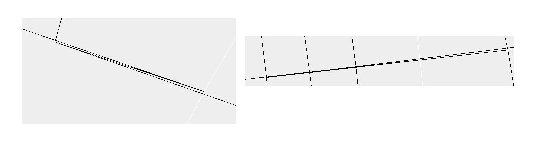
\includegraphics[scale=1.0]{routefailure.eps}
   \caption{Example Failures in Street Map}
   \label{fig:routefailure}
   \end{center}
\end{figure}
\section{Experimental Results}
\label{sec:results}
We repeated the \bmodb{} query execution several times for both data models and
approaches. The tables in figure \ref{fig:compruntimes} compare the average run times
query run times in seconds for the different scale factors, data models, and approaches.
As you can see the total run time of all queries in the network data model is around
50\% less than the total query run time of the \bmodb{} data model at each scalefactor.
\begin{figure}[h]
  \begin{minipage}{0.5\linewidth}
    \begin{tiny}
      \begin{tabular}{|c|r|r|r|r|}
        \hline
        &\multicolumn{4}{c|}{\textbf{Scalefactor 0.05}}\\
        \cline{2-5}
        &\multicolumn{2}{c|}{\textbf{BMODB}}&\multicolumn{2}{c|}{\textbf{Network}}\\
        \hline
        \textbf{Query}&\textbf{OBA}&\textbf{TBA}&\textbf{OBA}&\textbf{TBA}\\
        \hline
        \textbf{1}&0.086&0.100&0.090&0.113\\
        \hline
        \textbf{2}&0.003&0.003&0.003&0.002\\
        \hline
        \textbf{3}&0.346&0.345&0.112&0.568\\
        \hline
        \textbf{4}&9.105&15.403&0.142&1.303\\
        \hline
        \textbf{5}&1.076&1.623&0.927&1.377\\
        \hline
        \textbf{6}&16.781&14.934&5.004&4.483\\
        \hline
        \textbf{7}&2.996&3.007&1.221&6.790\\
        \hline
        \textbf{8}&0.346&0.424&0.225&0.213\\
        \hline
        \textbf{9}&99.375&193.929&22.935&24.349\\
        \hline
        \textbf{10}&139.795&36.636&81.770&84.298\\
        \hline
        \textbf{11}&0.143&0.111&0.158&0.898\\
        \hline
        \textbf{12}&0.297&0.133&0.228&0.202\\
        \hline
        \textbf{13}&11.284&7.341&1.159&1.336\\
        \hline
        \textbf{14}&0.525&0.727&0.793&3.734\\
        \hline
        \textbf{15}&1.201&0.802&0.625&0.543\\
        \hline
        \textbf{16}&43.567&5.346&0.680&1.579\\
        \hline
        \textbf{17}&1.084&0.935&0.234&0.337\\
        \hline
        \textbf{Total}&328.009&281.797&116.305&132.127\\
        \hline
      \end{tabular}
    \end{tiny}
  \end{minipage} \hfill
\begin{minipage}{0.5\linewidth}
    \begin{tiny}
      \begin{tabular}{|c|r|r|r|r|}
        \hline
        &\multicolumn{4}{c|}{\textbf{Scalefactor 1.0}}\\
        \cline{2-5}
        &\multicolumn{2}{c|}{\textbf{BMODB}}&\multicolumn{2}{c|}{\textbf{Network}}\\
        \hline
        \textbf{Query}&\textbf{OBA}&\textbf{TBA}&\textbf{OBA}&\textbf{TBA}\\
        \hline
        \textbf{1}&0.226&0.166&0.185&0.215\\
        \hline
        \textbf{2}&0.005&0.004&0.019&0.004\\
        \hline
        \textbf{3}&0.745&0.845&0.845&1.323\\
        \hline
        \textbf{4}&149.167&427.583&1.145&31.879\\
        \hline
         \textbf{5}&3.029&5.821&4.781&5.277\\
        \hline
        \textbf{6}&1463.214&5110.613&381.622&263.371\\
        \hline
        \textbf{7}&84.660&50.575&124.602&169.848\\
        \hline
        \textbf{8}&0.890&0.557&0.258&0.303\\
        \hline
        \textbf{9}&830.253&3153.720&120.470&156.693\\
        \hline
        \textbf{10}&4414.632&2015.096&2786.578&1791.941\\
        \hline
        \textbf{11}&0.656&0.914&6.030&7.738\\
        \hline
        \textbf{12}&36.210&0.213&0.274&0.267\\
        \hline
        \textbf{13}&119.685&94.366&29.126&36.086\\
        \hline
        \textbf{14}&10.912&3.915&36.041&38.552\\
        \hline
        \textbf{15}&30.874&18.711&10.317&7.989\\
        \hline
        \textbf{16}&35.490&8.655&0.584&1.969\\
        \hline
        \textbf{17}&82.242&343.826&0.550&8.026\\
        \hline
        \textbf{Total}&7262.888&11235.581&3503.429&2521.481\\
        \hline
      \end{tabular}
    \end{tiny}
  \end{minipage}\hfill
  \begin{minipage}{0.5\linewidth}
    \begin{tiny}
      \begin{tabular}{|c|r|r|r|r|}
        \hline
        &\multicolumn{4}{c|}{\textbf{Scalefactor 0.2}}\\
        \cline{2-5}
        &\multicolumn{2}{c|}{\textbf{BMODB}}&\multicolumn{2}{c|}{\textbf{Network}}\\
        \hline
        \textbf{Query}&\textbf{OBA}&\textbf{TBA}&\textbf{OBA}&\textbf{TBA}\\
        \hline
        \textbf{1}&0.146&0.123&0.082&0.092\\
        \hline
        \textbf{2}&0.003&0.003&0.004&0.003\\
        \hline
        \textbf{3}&0.456&0.523&0.134&0.834\\
        \hline
        \textbf{4}&32.832&80.881&0.217&7.504\\
        \hline
        \textbf{5}&1.539&2.824&1.768&2.251\\
        \hline
        \textbf{6}&70.266&120.294&20.605&14.884\\
        \hline
        \textbf{7}&14.479&10.423&10.107&35.036\\
        \hline
        \textbf{8}&0.435&0.446&0.202&0.225\\
        \hline
        \textbf{9}&237.581&485.998&41.579&50.853\\
        \hline
        \textbf{10}&605.718&139.565&378.248&309.345\\
        \hline
        \textbf{11}&0.233&0.149&0.178&3.017\\
        \hline
        \textbf{12}&4.332&0.160&0.269&0.260\\
        \hline
        \textbf{13}&30.173&13.791&5.737&5.248\\
        \hline
        \textbf{14}&1.115&1.166&1.469&9.286\\
        \hline
        \textbf{15}&8.824&4.286&2.644&2.084\\
        \hline
        \textbf{16}&29.389&5.500&0.376&0.847\\
        \hline
        \textbf{17}&8.453&4.169&0.306&0.923\\
        \hline
        \textbf{Total}&1045.974&870.300&463,926&442.691\\
        \hline
      \end{tabular}
    \end{tiny}
  \end{minipage}\hfill
  \begin{minipage}{0.5\textwidth}
      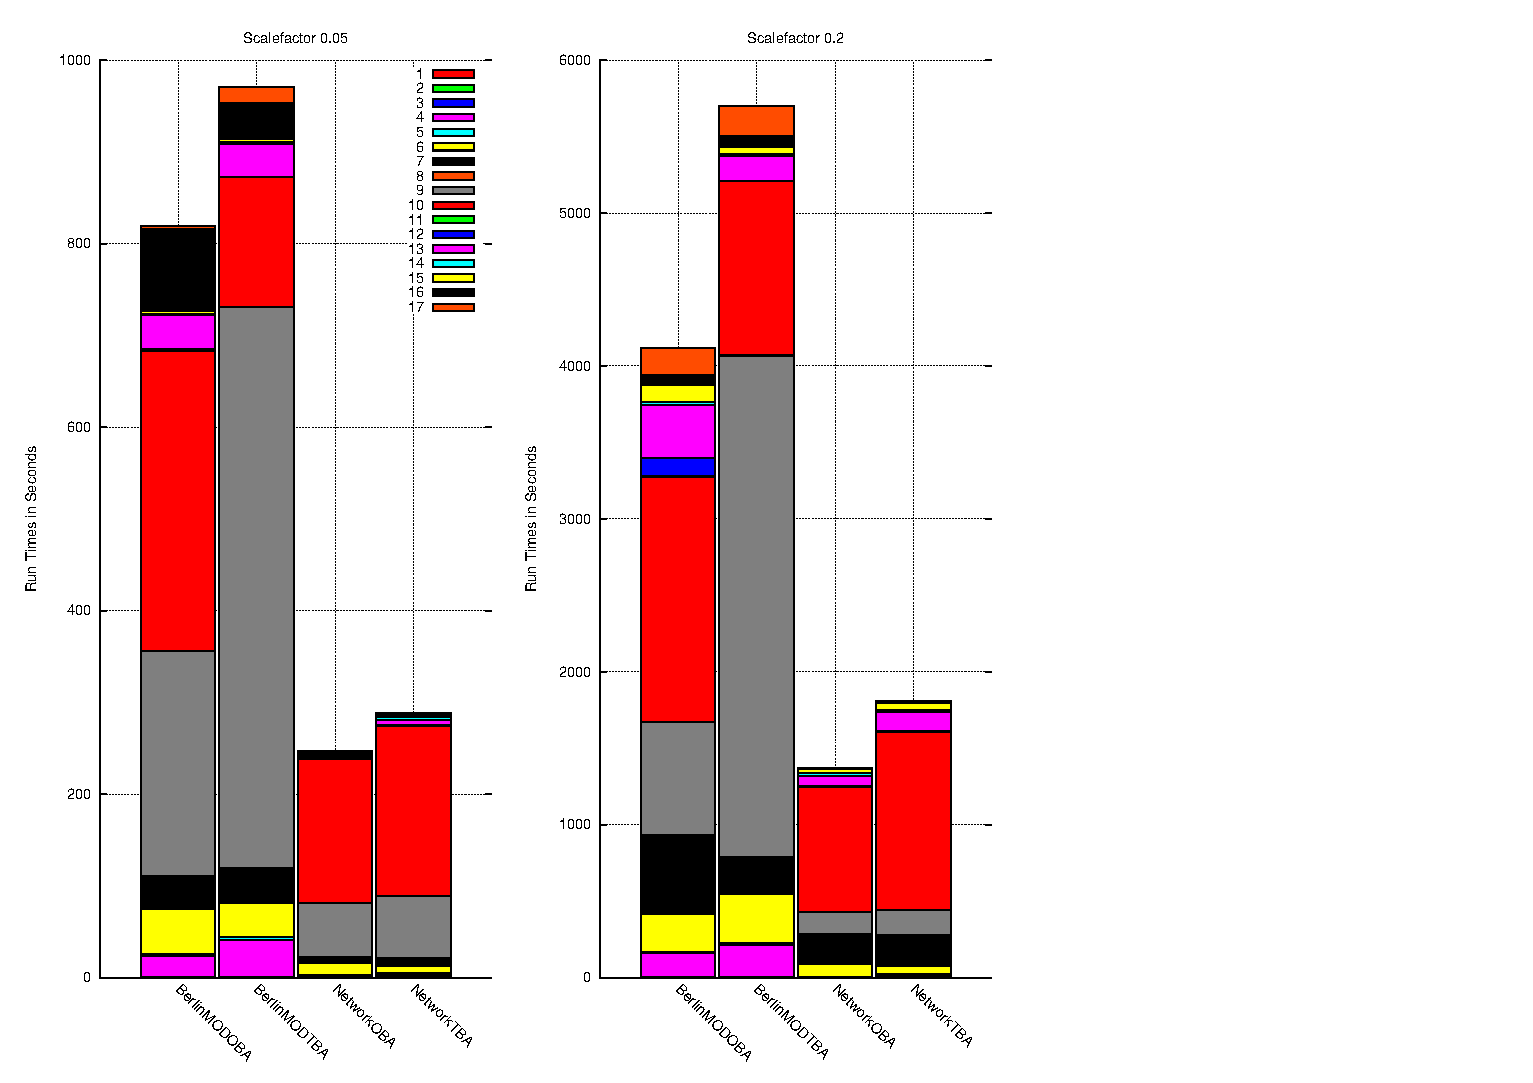
\includegraphics[width=1.0\linewidth]{compruntimesall.eps}
  \end{minipage}
 \caption{Compare Query Run Times in Seconds}
 \label{fig:compruntimes}
\end{figure}
For the queries 1 and 2 the query run times are almost the same for all data models
and approaches at the different scale factors. This is what we expected because
the both queries deal only with standard attributes and standard indexes, which
are not influenced by the different data models.

For query 3 the run times for all data models and approaches are very small. But
we can see a development of the ratio of the run times between the different
data amounts, data models and approaches. Although the query algorithms for both
data models and approaches is almost the same, the run time ratio for the different
data amounts is different. For the small databases (scalefactor 0.05 and 0.2)
the network database model outperforms in the OBA the data model of free movement
in two dimensional space, while for scalefactor 1.0 and all TBA queries the data
model of free movement in space outperforms the network data model. We think that
two different effects take place. On the one hand the number of units in the network
data model is less than the number of units in the data model of free movement in space,
such that the unit which contains the query time instant can be found faster.
On the other hand a \dt{gpoint} value has more internal elements (3 \dt{int}, 1 \dt{real},
and 1 \dt{bool}) than a \dt{point} value (2 \dt{real}, and 1 \dt{bool}), such
that result computing and copying is a little more expensive in the network data model.
The advantage of the smaller number of units in a binary search is smaller if
the number of units becomes bigger and the disadvantage of bigger results becomes
greater, that explains the different run time ratios for query 3.

In query 4 the network data model outperforms the data model of free movement in space
significantly at all scale factors (>2 min OBA, >6 min TBA at scalefactor 1.0).
The network data model index used in query 4
is much smaller (OBA 24 MB, TBA 160 MB, at scalefactor 1.0) than the
spatial unit index of the \bmodb{} (OBA 3.7 GB, TBA 3.7 GB at scalefactor 1.0)
and more precise, such that we don't need a additional refinement step after the
index usage in the network data model, like we do in the data model of free movement
in two dimensional space.

We expected the network data model to be slower than the data model of free
movement in two dimensional space, because we retranslate intermediate results
from the network data model representation into the \bmodb{} data model representation.
For the OBA this is correct. We need a little more time in the network data model
than in the data model of free movement in two dimensional space. But in TBA the
network data model outperforms the data model of free movement in two dimensional
space. This is due by the fact that a \dt{gline} value has less $route intervals$
than a \dt{line} value representing the same part of a curve has $half segments$,
such that the union of two or more \dt{gline} values in the aggregate step of query 5 in
TBA can be computed much faster than the union of two or more \dt{line} values.

The network data model outperforms the data model of free movement in space again
significantly at query 6 for
all data amounts and approaches, although we retranslate
intermediate results and use the distance function of the data model of free movement
in two dimensional space. In the network data model we reduce the number of candidate
pairs for the distance computation by pre selecting intersecting extended bounding boxes
and use the operation \op{notEverNearerThan} in OBA and TBA, while in the \bmodb{}
in the OBA no filtering is used and the computation is done by
\op{minimum}(\op{distance}($mp1$,$mp2$)$\leq$10.0), and in the TBA the operation
\op{spatialjoin} is used instead of bounding box intersection. While the operation
\op{distance} has always a run time from O($n$) the operation \op{everNearerThan}
stops computation immediately if the distance between two units is less than the
query value to reduce computation time. And the operation \op{spatialjoin} of the
\secondo{} DBMS seems to have a big weakness in implementation. Otherwise the
difference in the TBA query run times could not be so big (> 17 min OBA, > 80 min TBA,
at scalefactor 1.0).

After the very good results from query 4 we did not expect query 7 to have such
results in the run times comparison. In fact at scalefactor 1.0 the data model of free movement
in two dimensional space outperforms the network data model significantly in both
approaches and at all scale factors in TBA, while at the smaller scale factors in
OBA the network data model outperforms the the data model of free movement in
two dimensional space. We think there are two main causes on the one hand we
have to do the expensive operation \dt{at} for \dt{mgpoint} for the double number
of query \dt{gpoint} compared with the data model of free movement in space and
on the other hand the test points out a weakness of the network data model
implementation of the operation \op{at} for \dt{mgpoint}. But in the end network
data model looses at scalefactor 1.0 less than 45 seconds in the OBA respectively less
than 120 seconds in TBA, what is not much compared with the advantages in the
other benchmark queries.

Query 8 is a very fast query in both data models, although the query run time of
the network data model is more than 50\% less than the query run time of the
data model of free movement in two dimensional space. Which is caused by the
$length$ attribute of the \dt{mgpoint} and the smaller number of units of a
\dt{mgpoint} compared with the corresponding \dt{mpoint}.

For query 9 the network data model outperforms the data model of free movement
in space by orders of magnitudes the advantages named in the analysis of query 8's
run time results become a much higher impact when the number of examined trips
becomes bigger. At scalefactor 1.0 this saves more than 10 min time in the OBA and
more than 50 min time in the TBA.

The ratio of the run times of query 10 changes between the data amounts and the
both data models. In the OBA and at scalefactor 1.0 in the TBA the network data
model outperforms the data model of free movement in two dimensional space at
all scale factors, while in the TBA at the two small databases the data model of
free movement in two dimensional space outperforms the network data model significantly.
Before our experiments we expected that the \bmodb{} would outperform the network
data model in all cases, because of the expensive retranslation of intermediate
results. So why is the network data model faster (>20 min in OBA and >3 min in TBA
at scalefactor 1.0) than the data model of free movement in two dimensional space?
In the OBA we use bounding boxes for a preselect of candidate trips that step is not
performed in the \bmodb{}. In the TBA the results are only better for the big data
amounts we think this is due to the fact that the number of units in \dt{mgpoint}
values is always smaller than in \dt{mpoint} values such that the final aggregation
of the different trips of the same cars can be done faster in the network data model
than in the data model of free movement in two dimensional space.

Query 11 is identically with the first part of query 12 so it is surprising that
the run time of query 11 at scalefactor 1.0 is longer than the run time of query 12,
which does additional computations. In our experiments with the different queries
we have seen that there exist numerous cache effects depending on the sequence of
the queries. So we think that query 12 takes profit cache effects resulting from
query 11 running immediately before query 12. Another weakness of the network
data model pointed out by the run times of query 11 and query 14 is that our
network-temporal position index has bad run times for query $netbox$ objects constrained
from a single \dt{gpoint} and a single time instant. Which becomes more worse
with a higher number of indexed units. As you can see at query 15 this does not
hold for query $netboxes$ constrained from a single \dt{gpoint} and a time interval.
We have to spend some more work to figure out the problem and develop a better
network-temporal position index to improve our network data model system.

In our experiments we also tested the MON-Tree \cite{1046970} as network-temporal
index but the elapsed run time performance was not good, although the CPU run times
was very well.

The bad performance of the network-temporal position index is also shown by query 13.
The network data model outperforms the data model of free movement in two dimensional
space significantly, but we don't use any index in the executable network data model
queries, while the \bmodb{} uses its spatio-temporal index to preselect candidate
trips. The same holds for query 17.

The network data model version of query 16 takes profit from the smaller number
of units in the network data model and outperforms the data model of free movement
in two dimensional space.

Although we detected in our experiments some points of weakness in the network-temporal
position indexing, the network data model outperforms the data model of free movement in
two dimensional space by orders of magnitudes. The weakness of the network data model
almost occurs in queries with short run times, while the advantages of the network
data model take place in the queries with long run times, such that the weakness of
the network-temporal position index is covered by the advantages of the network
data model.
%\begin{figure}[H]
%\begin{center}
%   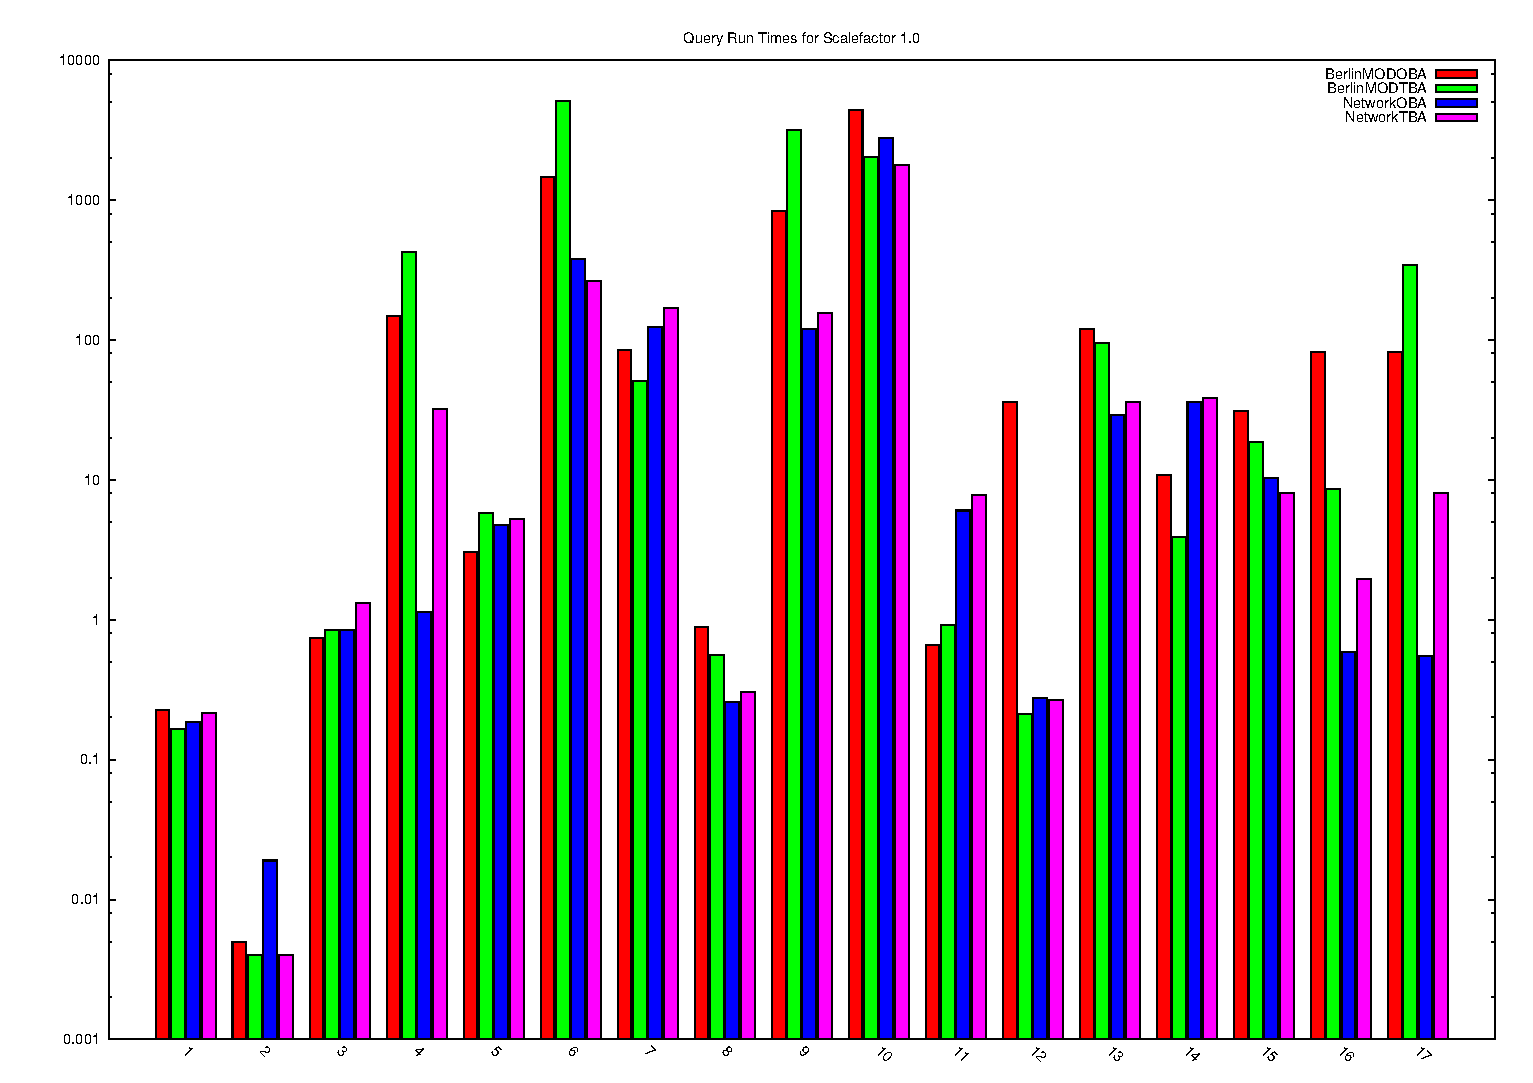
\includegraphics[width=1.0\textwidth]{compqueryruntimes.eps}
%   \caption{Compared Run Times for Each Query at Scalefactor 1.0}
%   \label{fig:compqueryruntimesall}
%\end{center}
%\end{figure}
%\section{New BerlinMOD Queries}
%\label{sec:newqueries}
\section{Summary and Future Work}
\label{sec:summary}
We presented our translation of the \bmodb{} into the network data model and
compared the capabilities of the both data models, with very good results for the
network data model. Our experiments show that the network data model outperforms
the data model of free movement in the two dimensional space by orders of magnitudes
with respect to storage space and query run times. This is manly caused by the much
lower number of units for a \dt{mgpoint} value compared with the number of units
of the corresponding \dt{mpoint}, which also results in smaller indexes for the
network data model objects. The \bmodb{} of the network data model pointed out
that we should spend time in the improvement of the network-temporal position index
and the \op{at} operation for \dt{mgpoint} and \dt{gpoint} values.

The good results of the network data model encourages us to work on a extension
of the \bmodb{}, which should enable us to compare the capabilities of different
spatio-temporal network data models with respect to the special challenges of
network data models, like shortest path and fastest path computation.

Another direction of our actual work is traffic flow estimation and traffic jam
representation in the network data model.

Other interesting themes for future work on the network data models is the efficient
computation of dynamic network distances between moving network objects.
\bibliography{BerlinMODAndNetworkDataModel}{}
\bibliographystyle{plain}
\end{document}
